\documentclass[varwidth=true, border=2pt]{standalone}
\usepackage{tkz-euclide}

\begin{document}
\usetkzobj{all}
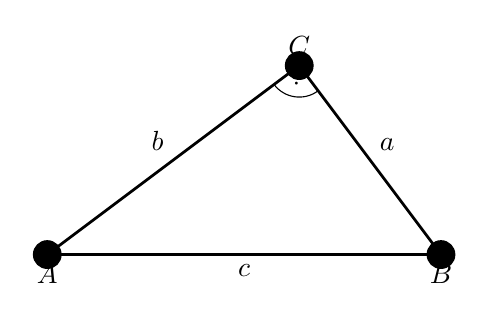
\begin{tikzpicture}
    \tkzSetUpPoint[shape=circle,size=10,color=black,fill=black]
    \tkzSetUpLine[line width=1]
    \tkzDefPoints{0/0/A, 5/0/B}
    \tkzInterCC[R,/tikz/overlay](A,4cm)(B,3cm) \tkzGetPoints{C}{D}
    \tkzDrawPolygon(A,B,C)
    \tkzDrawPoints(A,B,C)
    \tkzLabelSegment[below](A,B){$c$}
    \tkzLabelSegment[above left](A,C){$b$}
    \tkzLabelSegment[above right](B,C){$a$}
    \tkzLabelPoint[below](A){$A$}
    \tkzLabelPoint[below](B){$B$}
    \tkzLabelPoint[above](C){$C$}
    \tkzLabelAngle[pos=0.24](A,C,B){$\cdot$}
    \tkzMarkAngle[arc=l,size=0.4cm](A,C,B)
\end{tikzpicture}
\end{document}
